\documentclass{article}
\usepackage[utf8]{inputenc}
\usepackage{graphicx}
\graphicspath{ {./images/} }
\input{Packages.tex}
\usepackage{listings}
\usepackage[newfloat]{minted}
\usepackage{xepersian}
\usepackage{bidi}
\title{تمرین دوم امنیت سیستم های کامپیوتری }
\author{
امیررضا ویشته - 99522221
 و عرفان زارع - 98411432  }
\date{ابان 1402}    

\SetupFloatingEnvironment{listing}{name=برنامه}
\newcommand{\captionoflisting}[1]{\captionof{listing}{#1}}


\begin{document}

\maketitle

 \newpage
\section*{سوال اول تمرین ۱:}

امروزه بهترین \lr{cpu}  ها و \lr{gpu} های مرسوم در جامعه  و موجود قدرت محاسباتی حدود، 40 ترا فلاپس دارند.
برای مثال \lr{AMD Ryzen 9 5950X}  قدرت محاسباتی مغادل 749  گیگافلاپس دارد و این تعداد را در ثانیه محاسبه می نماید.

از طرفی \lr{gpu}  همچون  \lr{NVIDIA GeForce RTX 3090}  قدرت محاسباتی 35.6 ترا فلاپس را دارد .البته این اعداد بسته به شرایط و موقعیت و و بازدهی، میتواند کمتر هم باشد.
این درحالی است که سوپرکامپیوتر هایی همچون \lr{Fugaku}) ، قدرت محاسباتی حدود 442 پتافلاپس دارد.
(داده ها و نکات بیان شده در منابع موجود است و عکس بنچمارک \lr{cpu,gpu} اولیه، بدلیل عدم وضوح درست  تصویر، گذاشته نشده است ولی در لینک موجود می باشد.)
درمقام مقایسه دیگر، یک کارت گرافیک \lr{GeForce GTX 460} تقریباً 4 برابر عملکرد یک   \lr{CPU Core i5-2500K} را دارد . در این مورد \lr{GeForce GTX 460}  می‌تواند حدود 18,105 رمز عبور در ثانیه را با استفاده  بررسی کند، در حالی که\lr{ Core i5-2500K }تنها می‌تواند 4752 رمز عبور در ثانیه را بررسی کند.
برای حملات \lr{Brute-Force، GPU} ها به دلیل داشتن تعداد زیاد هسته‌های محاسباتی ، نسبت به \lr{CPU} (که معمولاً دارای چندین هسته است) سرعت بسیار بالاتری دارند.  این ویژگی باعث می‌شود GPU ها بتوانند عملیات رمزگشایی را با سرعت بسیار بالاتری انجام دهند. بنابراین، با توجه به توانایی‌های فعلی \lr{CPU و GPU}، می‌توان گفت که حملات \lr{Brute-Force} با سرعت بسیار بالاتر و کارآمدتری نسبت به گذشته انجام می‌شوند. البته باید توجه داشت که سرعت و کارآمدی این حملات به بسیاری از عوامل دیگر نظیر نوع رمز عبور و الگوریتم رمزگذاری نیز بستگی دارد و مسلما شکاندن رمز پیچیده، سختی و زمان بیشتری نیاز دارد.

 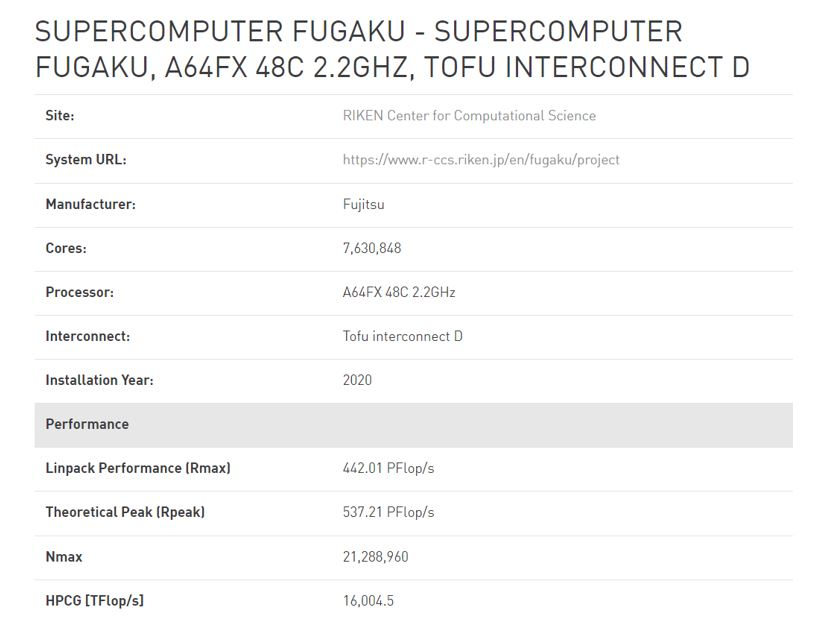
\includegraphics[width=12cm, height=10cm]{images/Capture.JPG}
 \lr{References }:
\begin{LTR}
\begin{itemize}
\item {\lr{https://www.top500.org/system/179807/}

\item \lr{https://gadgetversus.com/processor/amd-ryzen-9-5950x-specs/}
\item \lr{https://gadgetversus.com/graphics-card/nvidia-geforce-rtx-3090-specs/}
\item \lr{https://www.tomshardware.com/reviews/wireless-security-hack,2981-8.html}
\item \lr{f{https://securityboulevard.com/2022/05/brute-force-attacks-what-you-need-to-know/}}
\item \lr{{https://security.stackexchange.com/questions/118147/how-are-gpus-used-in-brute-force-attacks}}
\end{itemize}
\end{LTR}

\newpage
\section*{سوال دوم تمرین ۱}
در جنگ جهانی اول، آلمان ها از سامانه رمزگذاری \lr{"Transposition Double"} استفاده می‌کردند. این الگوریتم رمزگذاری به روش جابجایی اطلاعات و کلمات در متن اصلی بر اساس یک الگوی خاص اقدام می‌کند.
در این روش، ابتدا یک الگوی جابجایی مشخص می‌شود. سپس متن اصلی بر اساس این الگوی جابجایی مورد تغییر قرار می‌گیرد. در این جابجایی، هر قسمت از متن به جایگاه دیگری در متن منتقل می‌شود.
برای مثال، فرض کنید متن اصلی \lr{"HELLO WORLD"} باشد و الگوی جابجایی به صورت "2-5-3-1-4" تعیین شده باشد. در این صورت، ابتدا حرف اول به جایگاه دوم، حرف دوم به جایگاه پنجم، حرف سوم به جایگاه سوم، حرف چهارم به جایگاه اول و حرف پنجم به جایگاه چهارم منتقل می‌شوند. بنابراین، متن رمزگذاری شده به صورت \lr{"LHLOE LWRDO"} خواهد بود.
فواید این روش رمزگذاری این است که الگوی جابجایی به عنوان کلید رمزنگاری نقش ایفا می‌کند و تغییر الگوی جابجایی می‌تواند باعث تولید رمزهای متفاوت شود. این روش به دلیل سادگی ، آسیب‌پذیری ‌زیادی نیز دارد و به راحتی قابل شکستن است. در ادامه جنگ جهانی اول، روش‌های قوی‌تری برای رمزنگاری معرفی شدند و استفاده از \lr{"Transposition Double"} کم شد.
رمزگذاری جابجایی شامل جابجایی حروف یا مجموعه ای از متن است تا پیامی مخفی شود. در حالت \lr{Transposition Double}، متن بر اساس یک الگوی خاص و مشخص جابجا می‌شود


فرایند رمزگذاری با استفاده از \lr{Transposition Double} با انتخاب یک الگوی جابجایی  انجام می شود. این الگو مشخص می‌کند که چگونه متن اصلی قرار است رمزگذاری شود. الگو می‌تواند یک دنباله اعداد یا هر نوع دستور دیگری باشد.

بعد از تعیین الگو، متن اصلی بر اساس الگوی جابجایی تغییر شکل می‌یابد. هر بخش از متن بر اساس دستورات الگو به یک موقعیت دیگر در متن منتقل می‌شود. این بازترتیب دادن معمولاً به صورت مرحله به مرحله و به ترتیب متن انجام می‌شود.

برای رمزگشایی پیام، گیرنده نیاز به دانستن الگوی جابجایی استفاده شده برای رمزگذاری دارد. با اعمال الگوی جابجایی معکوس، متن می‌تواند به حالت اصلی خود برگردانده شود.



\newpage
\section{تمرین ۱: سوال سوم}

در ابتدا، تعداد هر یک از حروف زبان انگلیسی در متن را محاسبه می نماییم که کد آن در فایل پیوست موجود است. آنگاه با توجه به اینکه الگوریتم رمزنگاری متن ، از نوع مستوی هست ، پس الگوریتم ما به شکل $AX+B=\{\text{$alphabet$}\} \mod 26$ است . ما میدانیم حروف پرتکرار در زبان انگلیسی، شامل$A,E,C$ می باشند. پس ابتدا ، مقادیر پرتکرار ترین حروف هارا مطابق آن ها درنظر میگیریم. سپس با توجه به آنکه متن ما با جایگذاری این حروف تاحدی داری معنا شد،( در تعداد کمی از حرف های دو تا سه حرفی، یا کلماتی پرتکرار در نگارش متن) انگاه می آییم و بررسی میکنیم که آیا اگر مقادیر $A,B$ موجود در فرمول،را با استفاده از دو حرف $A,E$ محاسبه نماییم ، ابتدا به مقادیر و خروجی می رسیم؟ (مقادیری ما به ازای آن ها هست؟) و سپس به سراغ جایگذاری اعداد و فرمول ها و به دست آوردن کلمات دیگر میرویم. درنهایت طبق توضیحات بالا، هرکدام از حروغ کلید که به همراه تکرارشان در سمت راست آمده اند، معادل حروف سمت چپ اند. مقدار $A=3$ و $B=10$ می باشد .

\begin{align*}
K: & 58 & \rightarrow & A \\
W: & 52 & \rightarrow & E \\
Q: & 47 & \rightarrow & C \\
X: & 47 & \rightarrow & N \\
J: & 46 & \\
P: & 41 & \\
T: & 42 & \\
R: & 38 & \\
I: & 36 & \\
M: & 32 & \rightarrow & S \\
A: & 30 & \\
D: & 26 & \rightarrow & P \\
N: & 19 & \\
E: & 19 & \\
U: & 18 & \\
Z: & 18 & \\
V: & 18 & \\
C: & 17 & \rightarrow & G \\
F: & 16 & \\
B: & 12 & \rightarrow & X \\
Y: & 11 & \\
S: & 10 & \\
O: & 5 & \\
G: & 1 & \\
H: & 0 & \\
L: & 0 & \\
\end{align*}

در نهایت با جایگذاری نکات بالا در متن ، به خروجی با معنای زیر میرسیم.
\begin{LTR}



\lr{Plain\_text:}

\lr{g is expected to support data rates of terabyte per second this level of capacity and latency will be unprecedented and will extend the performance of g applications along with expanding the scope of capabilities in support of increasingly new and in novative applications across the realms of wireless connectivity cognition sensing and imaging g higher frequencies will enable much faster sampling rates in addition to providing significantly better throughput and higher data rates the combination of sub mm wave eg wave lengths smaller than one milli meter and the use of frequency selectivity to determine relative electromagnetic absorption rates is expected to lead to potentially significant advances in wireless sensing technology additionally where as the addition of mobile edge computing is a point of consideration as an addition to g networks mobile edge computing will be built in to all g networks edge and core computing will be come much more seamlessly integrated as part of acombined communications computation infrastructure framework by the time g networks are deployed this will provide many potential advantages as g technology becomes operational including improved access to artificial intelligence capabilities.}
\end{LTR}

\end{document}